\documentclass[10pt,conference,a4paper]{IEEEtran}

\usepackage{hyperref}
\usepackage{graphicx}	% For figure environment
\usepackage{amsmath}
\usepackage{amssymb}
\usepackage{subcaption}
\usepackage[normalem]{ulem}
\useunder{\uline}{\ul}{}

\newcommand*\desc[1]{\item[\textbf{#1}]}

\begin{document}
\title{Road Segmentation}
\author{
  Beuchat Bastien, Mamie Robin, Mion Jeremy\\
  \textit{CS-433: Machine Learning (Fall 2019),}\\
   \textit{École Polytechnique Fédérale de Lausanne, Switzerland}
}

\maketitle

\begin{abstract}
This report presents the different methods we used to solve the problem of road segmentation out of satellite images.
Convolutional neural networks are shown to be very efficient for this task, and we can cite U-Net \cite{unet} as one of the best performers.
Such networks require considerable amounts of input data, which were not provided in this case.
As such, methods of expanding the original data set were tested to help us reach a better accuracy.
The best result was achieved using a CNN based on UNet++, yielding a final official F1-score of \textit{0.906}.
\end{abstract}

\section{Introduction}

Image segmentation is a computer vision process in which images are partitioned into different segments.
It has a key role to play in many different fields of research.
Among its concrete applications are domains such as medical imaging, machine vision and in our case dynamic map creation.
Acquiring aerial photography is a cheap and efficient way of collecting information about the topography of the terrain below.
In this project, we create a machine learning algorithm that detects the roads out of these photographs.
Automatically detecting the location and width of roads is a very powerful tool that allows map-making companies to keep their data up to date with very little cost.

Road segmentation, in this context, is not trivial.
On the one hand, roads are not always clearly distinguishable from the rest of the topography.
For example, cars, trees, buildings and shadows may partially hide them.
On the other hand, other structures such as roofs, train tracks and car parks may look like roads.
They should thus ideally not be detected as such.

In this project, we explore the different possibilities by starting with a simple convolutional neural network, and ending up with one implementing UNet++ using deep supervision \cite{unet++}.

\section{Data Analysis}
\label{data_analysis}

To act as training data, 100 satellite images were provided.
These images are 400$\times$400 pixels in size, each pixel consisting of three channels (figure \ref{fig:aerial}).
To label which pixel is a road, another set of 100 images is given, named ground truths.
They consist of black and white images (figure \ref{fig:gt}), acting as a mask of the aerial images.

\begin{figure}[ht]
  \begin{subfigure}[b]{0.2\textwidth}
    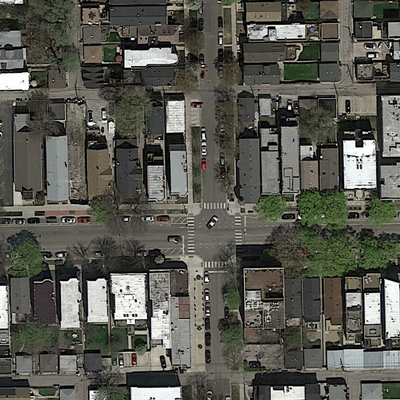
\includegraphics[width=\textwidth]{project2/report/images/image.png}
    \caption{Aerial image}
    \label{fig:aerial}
  \end{subfigure}
  %
  \begin{subfigure}[b]{0.2\textwidth}
    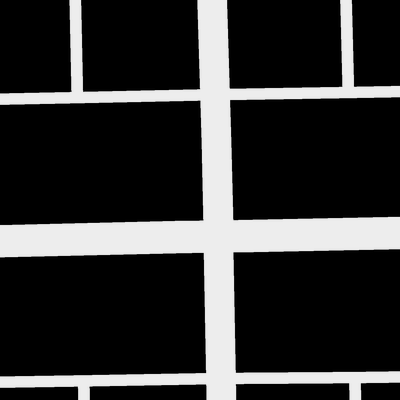
\includegraphics[width=\textwidth]{project2/report/images/groundtruth.png}
    \caption{Ground truth}
    \label{fig:gt}
  \end{subfigure}
  \centering
  \caption{Example image from the training set}
\end{figure}

Although these images are precisely labelled, the end goal is to provide more coarsely-grained results.
Indeed, the expected result is to label the test set using 16$\times$16 patches of pixels, which is composed of images containing 600$\times$600 pixels.
These patches indicate a binary result, not a probabilistic one: either they signal a road, or they do not.
Thus, the decision threshold is important for the final road detection, and has to be taken into account.
Fine tuning of this threshold is further discussed in section \ref{prediction}.
% TODO talk about what the images really are, i.e. shitty roads with different gradients of colour, can be easily confused with roof tops, etc. (more in depth than in the introduction, but I think it would have its place here

To mitigate the issues that come with the definition of a road on these images, we use convolutional neural networks, which are well suited for image recognition in general.

\section{Data Preprocessing}

As discussed in section \ref{data_analysis}, images in our training set are rather scarce -- for a convolutional neural network.
We have come up with a solution to expand it almost \textit{ad infinitum}.
This preprocessing avoids any over-fitting in our final network, which would arise if no other preparation was done on the data.

\subsection{Rotation and symmetry}
\label{rot_sym}

As a first attempt, a D4 dihedral symmetry was used to expand the original training set from 100 to 800 images.
The basics of the D4 dihedral expansion can be seen in figure \ref{fig:d4Dyhedral}.
Unfortunately the image expansion did not suffice to avoid over-fitting the model.

\begin{figure}[htpb]
    \centering
    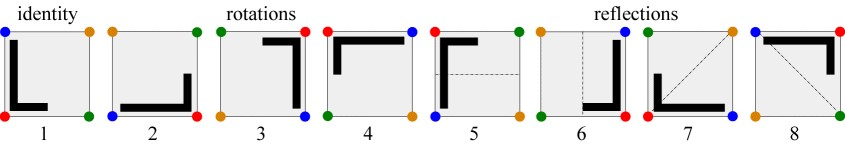
\includegraphics[scale=0.37]{project2/report/images/symmetries.jpg}
    \caption{D4 Dihedral set. Illustration from \cite{d4Dihedral}}
    \label{fig:d4Dyhedral}
\end{figure}

\subsection{Automated data augmentation}
\label{augm}

The \textit{Keras} library \cite{keras} provides a variety of very useful preprocessing functions.
\textit{ImageDataGenerator} allows us to define a number of parameters.
To yield an image, this generator then randomly assigns a value in the range defined for each of these parameters, for a given image of our training set.
This is repeated 100 times for each of our 100 images, generating 10'000 images in total.
Here are the parameters defined, as well as their possible ranges:

\begin{description}[\IEEEsetlabelwidth{\textbf{Brightness }}]
    \desc{Rotation} Rotates the image in a 0 to 360 degrees range
    \desc{Zoom} Zooms either in or out the image until a factor of 0.3 at most
    \desc{Brightness} Dims the image by 30\% at most
    \desc{Shifting} Shifts the image by a factor of 0.1 in each direction at most
    \desc{Flipping} Flips the image horizontally or vertically, or does nothing
    \desc{Shearing} Shears the image by a factor of 0.15 at most
\end{description}

\begin{figure}[ht]
  \begin{subfigure}[b]{0.2\textwidth}
    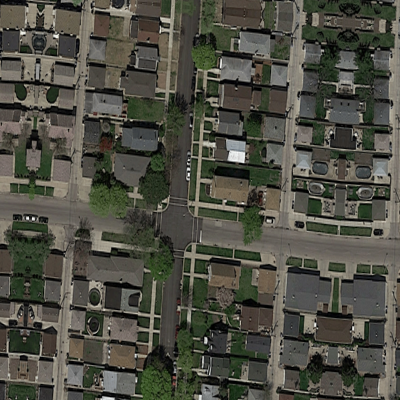
\includegraphics[width=\textwidth]{project2/report/images/satImage_001_0_1476.png}
    \caption{Aerial image extended}
    \label{fig:aerial_extended}
  \end{subfigure}
  %
  \begin{subfigure}[b]{0.2\textwidth}
    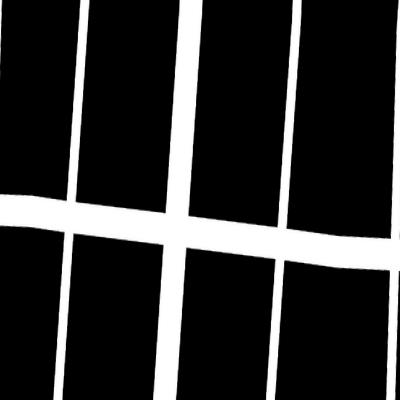
\includegraphics[width=\textwidth]{project2/report/images/groudtruth_extended.png}
    \caption{Ground truth extended}
    \label{fig:gt_extended}
  \end{subfigure}
  \centering
  \caption{Example of an image and its ground truth from our extended set. Notice that the sides of the image show some symmetry, due to the generator reaching outside of the predefined image.}
  \label{fig:ext}
\end{figure}

If any data is missing -- e.g. when shifting the image \mbox{--,} the function simply reflects the image symmetrically -- see figure \ref{fig:ext}.
With this method, the training set is completely new, and no image is exactly the same.
We call this newly generated set the augmented (training) set.

We see on figure \ref{fig:val_acc} that the accuracy of the validation set on a U-Net -- see section \ref{sec:unet} -- trained with this newly created data set very quickly outperforms the training done with our first data augmentation and remains very stable.
This is understandable by the fact that the second method allows us to create much bigger data sets.
Based on this result, our models are trained using this data augmentation technique.

\begin{figure}[ht]
    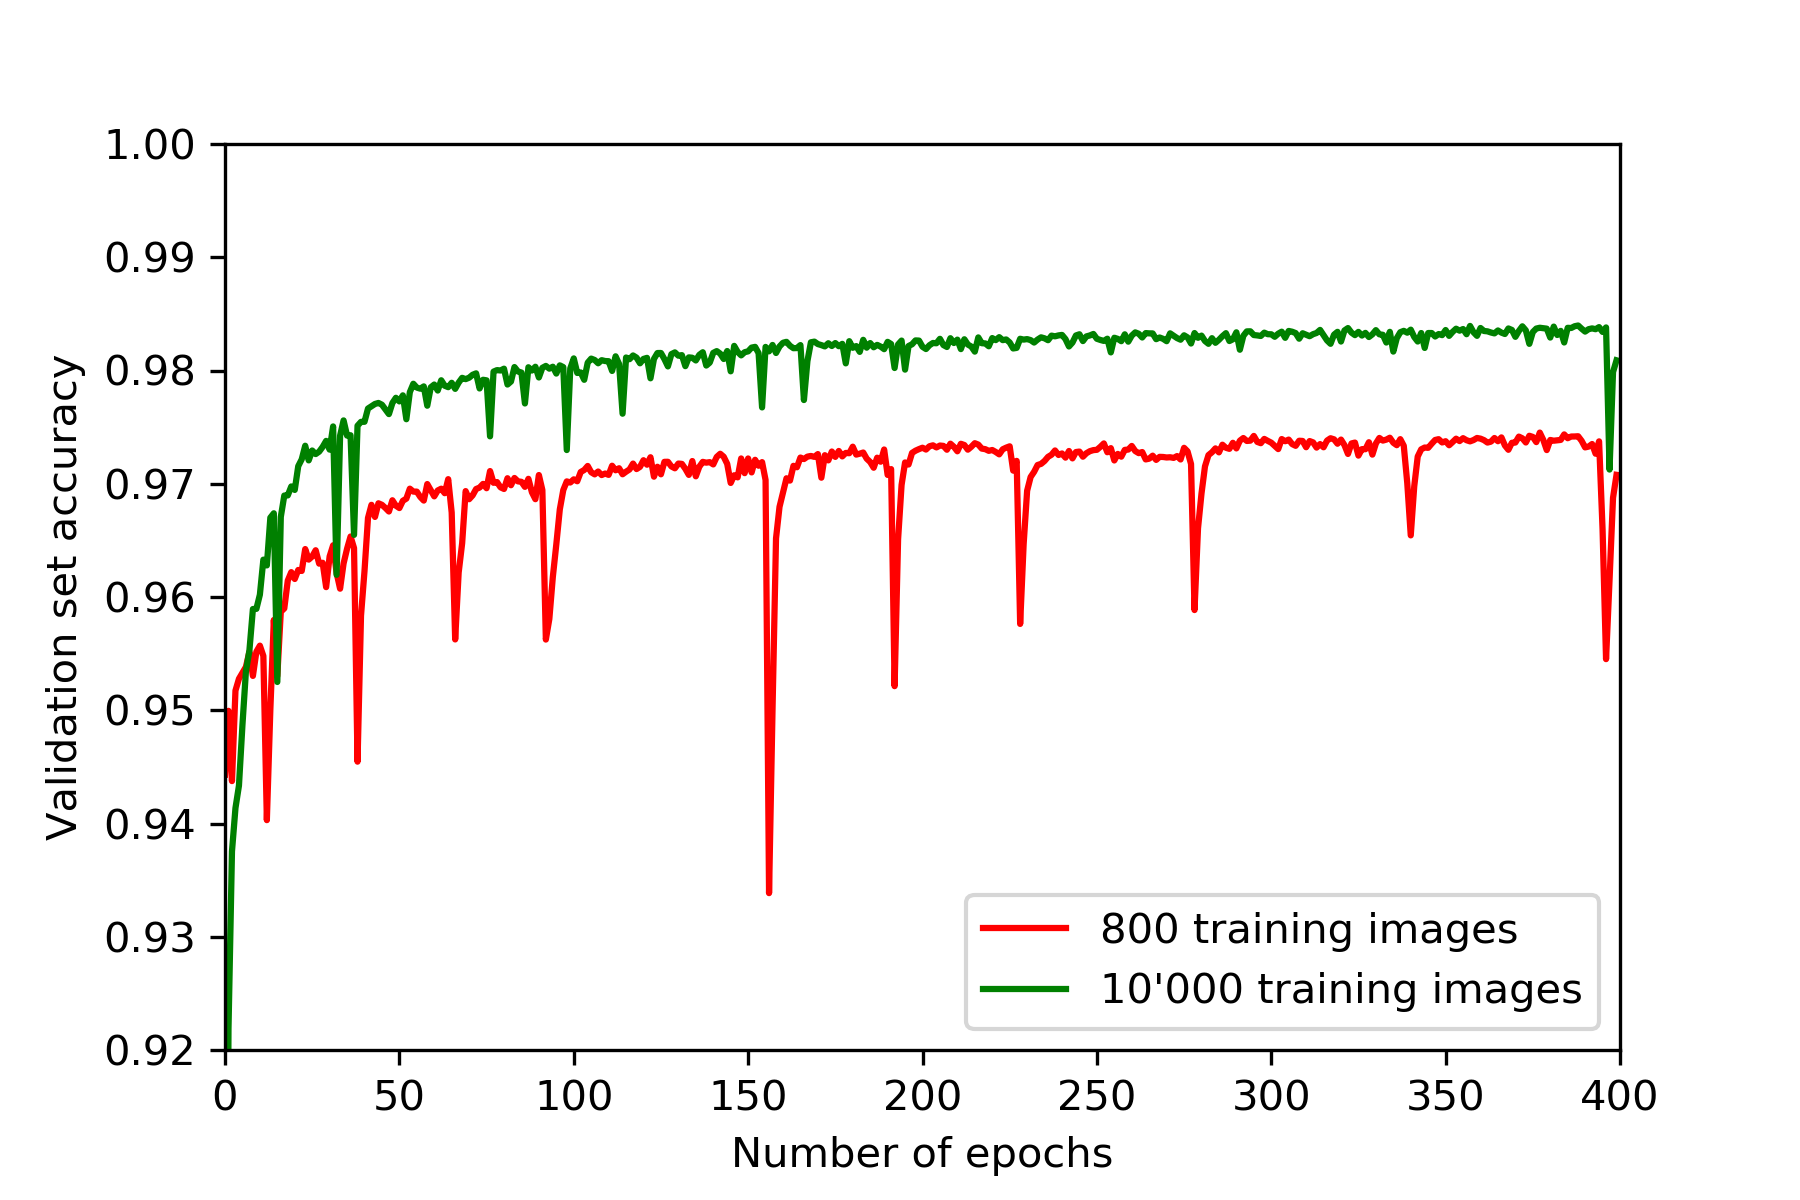
\includegraphics[width=0.5\textwidth]{project2/report/images/validation_graph.png}
    \caption{Comparison of a U-Net trained for 400 epochs using the augmented sets talked about in sections \ref{rot_sym} (800 images) and \ref{augm} (10'000 images). The validation set represents 10\% of the data set.}
    \centering
    \label{fig:val_acc}
\end{figure}

\section{Models}
\label{Models}

As previously mentioned, the task of image segmentation is nowadays done very successfully using convolutional neural networks \cite{cnn_seg}.
Today's state of the art fully conventional neural network for image segmentation is U-Net, originally developed in 2015 for biomedical image segmentation and proving itself very powerful for general purpose imagery.
Starting from a basic CNN, we then go through different iterations of U-Net.
All our U-Net versions use the optimiser named Adam \cite{kingma2014adam} that is very popular nowadays in computer vision.
It is well suited for a large number of parameters and it does not require a lot of tuning.
The binary cross-entropy loss function, a standard loss function, is used, with the notable exception of the model where an hybrid loss function is implemented.

\subsection{Basic CNN}

The first task is getting a baseline with a simple CNN provided as a starting point to the competition.
The accuracy and F1 score of the CNN are used as a baseline to compare the other more advanced algorithms.
The architecture of the basic CNN is composed of two 2D convolutions with rectified linear units (ReLU) and max-pooling before a fully connected hidden layer.
The fully connected hidden layer is finally fully connected to the output layer.   

\subsection{U-Net}
\label{sec:unet}

Typically, CNNs are used for image classification, where given an image a single label must be predicted.
Many biomedical applications rather have a label per pixel.
U-Nets have yielded promising results on medical image segmentation.
By avoiding fully connected layers and by using the ReLU activation function, U-Nets manage to be quite complex models while keeping the computation costs quite low.
Dropout layers are included in the model so as to counteract the tendency of the model to over-fit the training data, yielding a fragile model \cite{dropout}.

\begin{figure}[ht]
\centering
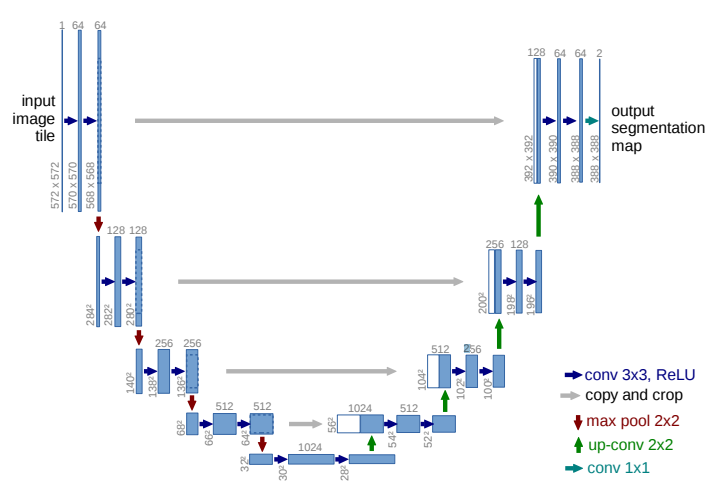
\includegraphics[scale=0.45]{project2/report/images/Unet.PNG}
\caption{U-net architecture (example for 32x32 pixels in the lowest resolution).
Each blue box corresponds to a multi-channel feature map.
The number of channels is denoted on top of the box.
The x-y-size is provided at the lower left edge of the box.
White boxes represent copied feature maps, and the arrows denote the different operations.
Source: \cite{unet}}
\label{unet_arch}
\end{figure}

Our network differs from the one shown in figure \ref{unet_arch} by the input dimension that is of 400$\times$400. 
The lowest dimension of our U-Net is 25$\times$25.

\subsection{UNet++}

Recent work on image segmentation extended the U-Net model to UNet++.
This architecture was proposed in the context of medical image segmentation with the aim of having a more powerful architecture.
The skip pathways are re-designed with dense layers. 
All layers are activated with the ReLU activation function.
Since it has been shown that UNet++ can beat U-Net for some tasks of medical image segmentation, it is worthwhile to test the UNet++ architecture on the problem of road segmentation. 
This model is slower than U-Net with respect to both training time and prediction time but could potentially achieve a better accuracy.

\begin{figure}[ht]
\centering
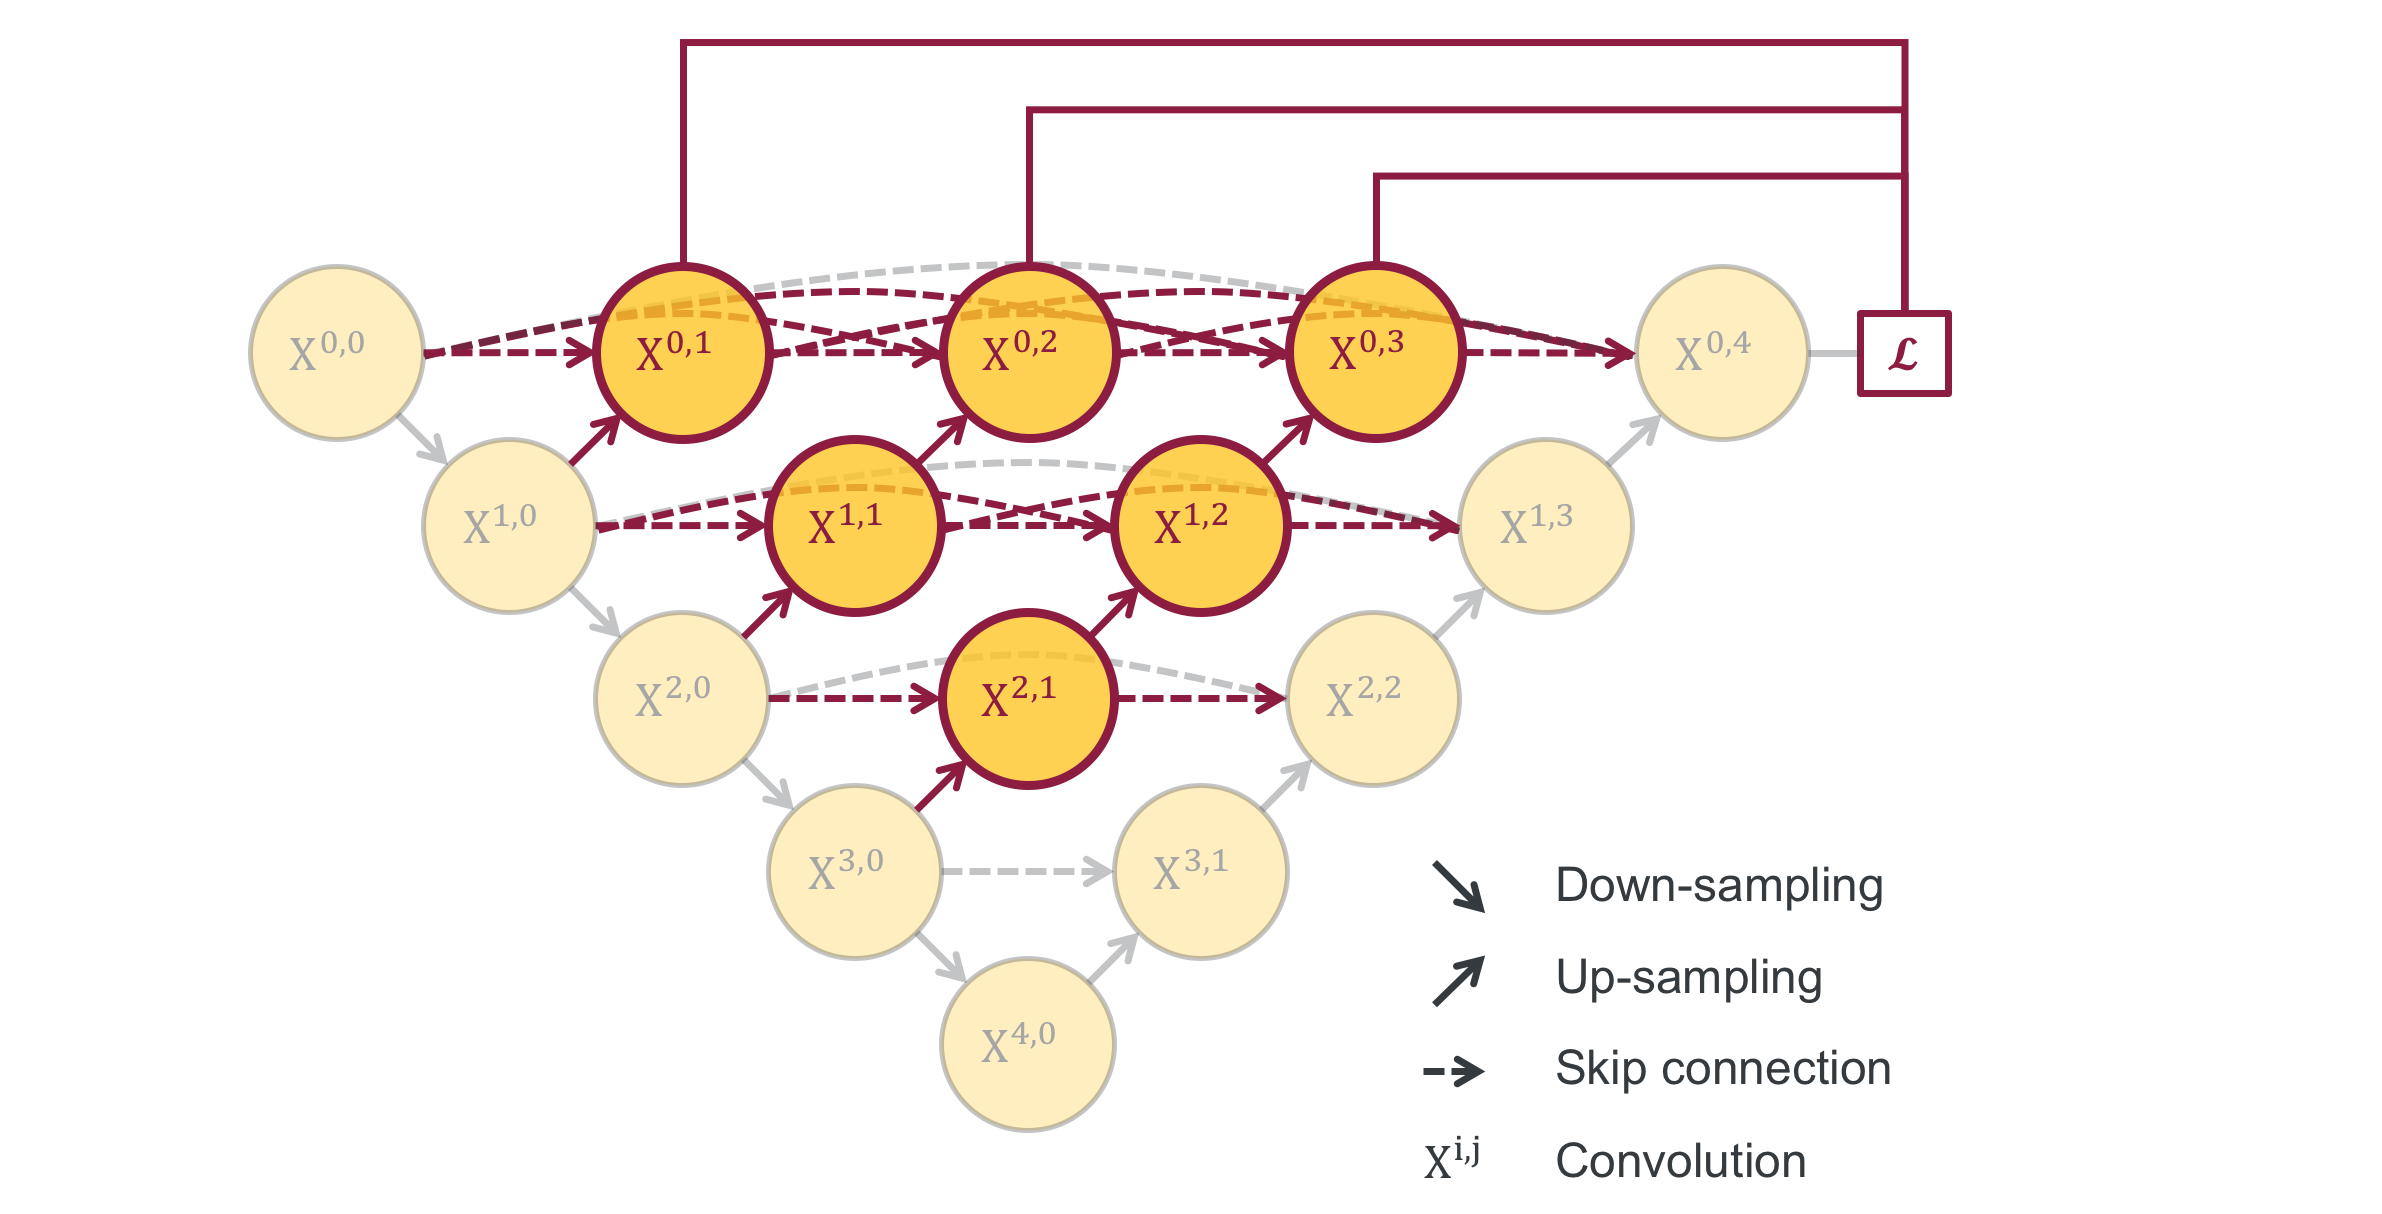
\includegraphics[scale=0.2]{project2/report/images/UNet++.PNG}
\caption{UNet++ architecture with deep supervision. Source: \cite{unet++}}
\label{unet++_arch}
\end{figure}

\subsubsection{No supervision}

The previous network is adapted to this architecture following strictly the instructions of the original UNet++ paper -- see figure \ref{unet++_arch}.
In a first test run, we did not implement the deep supervision and used the binary cross-entropy as loss function.

\subsubsection{Deep supervision}
\label{sec:deep supervision}

Deeply-supervised nets were first proposed in 2014 \cite{lee2014deeplysupervised}, as well as by the authors of UNet++.
They experimentally demonstrated that deep supervision can improve accuracy of UNet++ for some tasks.
To achieve deep supervision, three outputs are added to UNet++; our implementation follows the way explained in an additional paper also written by the UNet++ authors \cite{zhou2019unet}.
We add three 1$\times$1 convolutions with a sigmoid activation function as output.
These layers are directly linked to the inner dense layers of the UNet++. 
They also use a hybrid loss function.
In this project, we test two loss functions: binary cross-entropy and a hybrid loss function.
The hybrid loss function is a combination of the binary cross-entropy loss function and dice coefficients as proposed by the authors of UNet++.


\section{Predictions} \label{prediction}

The provided test set is composed of 600$\times$600 images.
It sets the constraint of being able to predict a bigger image than those of the training set.
Indeed, the training set is composed of 400$\times$400 images. 
This constraint does not add anything to our baseline CNN as some preprocessing is done before the actual network is run to cut the image in patches of 16$\times$16.
On the other hand, the input of the U-Net and UNet++ implementations are the full 400$\times$400 training images.
Therefore, the U-Net and UNet++ can use more of their surroundings to determine a label.
This has an implication that we can only evaluate these models on 400$\times$400 inputs.
For a better robustness of our code, we use an external library to solve this problem \cite{blend}.

This library makes tiles of size 400$\times$400, creates the D4 dihedral group of the tile and then gets the prediction images of the D4 dihedral group before merging them back together by reversing the symmetry and rotations.
This technique ensures that the orientation of the image is irrelevant during the prediction process.

We observe that changing the decision threshold could improve our predicted picture.
Therefore, all the predicted images are stored as the output of the model without applying a binary decision on whether each pixel is a road or not. 
This allows for more efficient post processing since no data is lost in a binary decision.
Each model outputs an image that represents the probability that each pixel is a road. 
Using the metric discussed in part \ref{sec:F1 metric}, we grid-search the optimum value to minimise this hyper-parameter.
We use a separate set of generated images as a validation set for this purpose.

\begin{figure}[ht]
  \begin{subfigure}[b]{0.2\textwidth}
    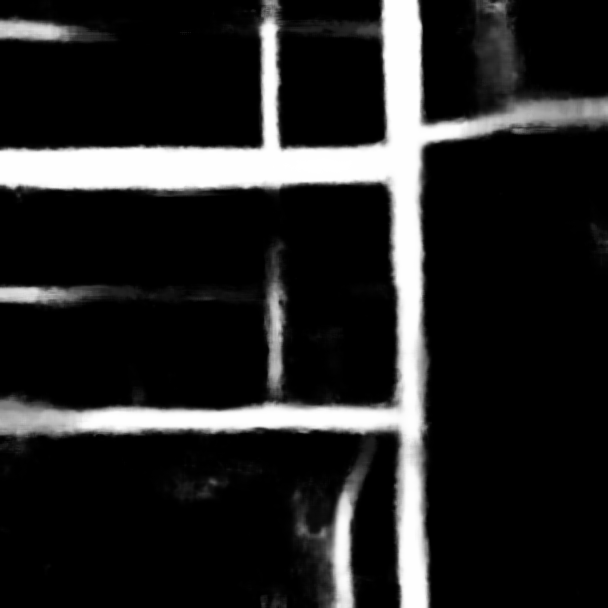
\includegraphics[width=\textwidth]{project2/report/images/gt_12.png}
    \caption{Prediction 1}
    \label{fig:gt1}
  \end{subfigure}
  %
  \begin{subfigure}[b]{0.2\textwidth}
    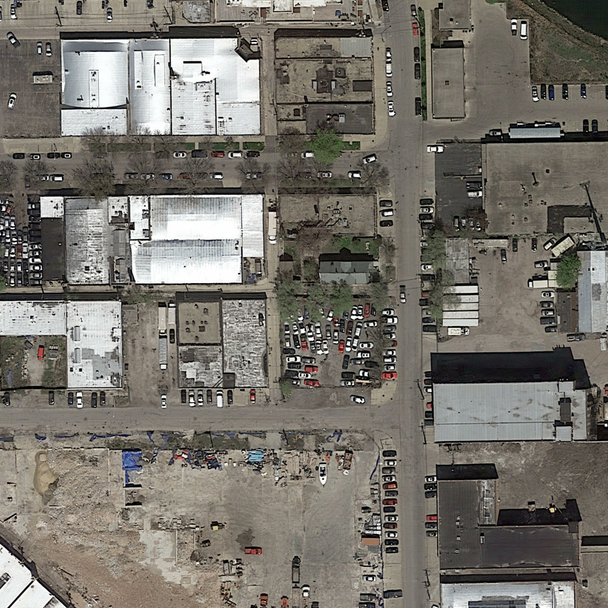
\includegraphics[width=\textwidth]{project2/report/images/test_12.png}
    \caption{Aerial image 1}
    \label{fig:aerial1}
  \end{subfigure}
  %
  \begin{subfigure}[b]{0.2\textwidth}
    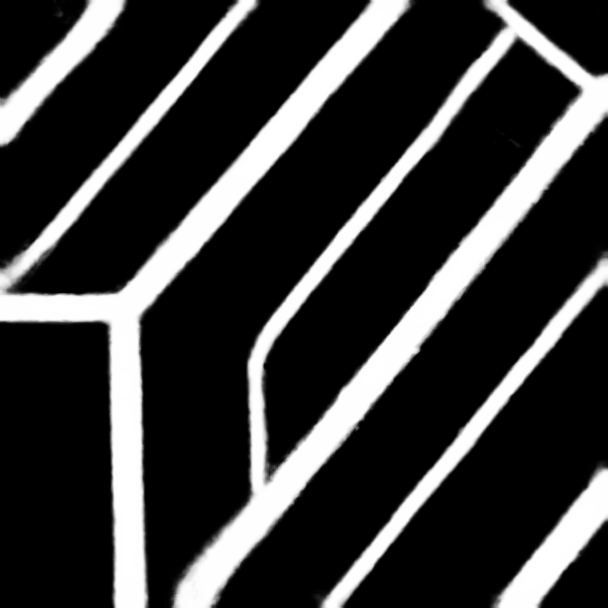
\includegraphics[width=\textwidth]{project2/report/images/gt_48.png}
    \caption{Prediction 2}
    \label{fig:gt2}
  \end{subfigure}
  %
  \begin{subfigure}[b]{0.2\textwidth}
    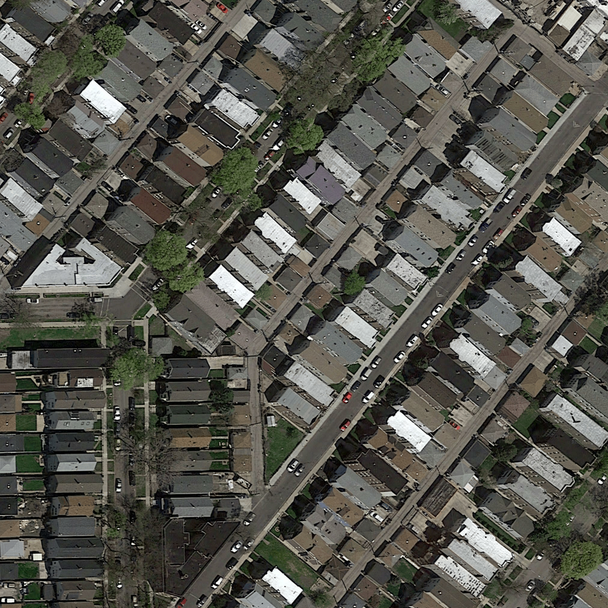
\includegraphics[width=\textwidth]{project2/report/images/test_48.png}
    \caption{Aerial image 2}
    \label{fig:aerial2}
  \end{subfigure}
  \centering
  \caption{Example of predictions with UNet++ done on two images from the test set.
  This model trained for 100 epochs on our augmented set.}
  \centering
\end{figure}

\section{Results}

The best results for the models described in section \ref{Models} are shown in table \ref{tab:results}.
All the models\footnote{\label{foot:baseCnn}All except for the baseline CNN that was trained on the D4 dihedral image expansion set (800 images).} are trained on an augmented data set of 10000 pictures. 

Cross-validation is applied with a split of 0.1, meaning that 9000 pictures are used to train the model and 1000 pictures during the validation process.
Batch size varied from model to model.
Models are trained on the largest batches possible without having to pay the extra computational cost.
The UNet++ DS\footnote{DS is short for deep supervision.} has very large memory requirements, forcing the batch size to one.

\subsection{Metrics}

Two metrics are devised to determine if our models are improving.
In both of these metrics, we decided to calculate a low resolution image, as the submission format for the challenge is requesting.
Each 16$\times$16 patch is converted to a single pixel.

\subsubsection{Average number of miss-classified tiles}

The average number of miss-classified tiles give us a precision score that does not take into account the imbalances between predicted classes.

\subsubsection{F1 on validation set}
\label{sec:F1 metric}

The F1 score gives us a better metric that takes into account the imbalances between the predicted classes.
Hence, this one is more relevant to our problem, since there are fewer patches representing roads than not.

\begin{table}[h!]
\begin{tabular}{|c|c|c|c|c|c|}
\hline
\multicolumn{1}{|l|}{} & \textbf{\begin{tabular}[c]{@{}c@{}}Baseline \\ CNN*\end{tabular}} & {\ul \textbf{U-Net}} & {\ul \textbf{UNet++}} & \textbf{\begin{tabular}[c]{@{}c@{}}UNet++ \\ DS\end{tabular}} & \textbf{\begin{tabular}[c]{@{}c@{}}UNet++ \\ DS \\ hybrid \\ loss \end{tabular}}\\
\hline
\textbf{F1 AIcrowd} & 0.701 & 0.905 & \textit{0.906} & 0.883 & 0.820\\
\hline
\textbf{\begin{tabular}[c]{@{}c@{}}avg \# tiles\\ misclassified\end{tabular}} & 126.1 & 9.96 & \textit{10.03} & 19.04 & 58.29\\
\hline
\textbf{F1 val. set} & 0.695 & 0.968 & \textit{0.968} & 0.937 & 0.819 \\
\hline
\textbf{\# of epoch} & 100 & 400                  & \textit{100}          & 50                                                             & 50                                                                         \\ \hline
\textbf{Batch size}                                                           & 16                                                                & 32                   & \textit{4}            & 1                                                              & 1                                                                          \\ \hline
\textbf{\begin{tabular}[c]{@{}c@{}}Decision\\ threshold\end{tabular}}         & 0.25                                                              & 0.358                & \textit{0.400}        & 0.445                                                          & 0.535                                                                      \\ \hline
\textbf{\begin{tabular}[c]{@{}c@{}}Training\\ run time\end{tabular}}          & 30min                                                             & \textit{7h}          & \textit{17h}          & 9h30                                                           & 9h30                                                                       \\ \hline
\end{tabular}
\centering
\caption{For run time estimates, all models were trained with a computer having \textit{i9-9900k 5GHz, 64GB RAM, RTX 2080 Ti}. The UNet++ yielded the best results with the U-Net close behind.}
\label{tab:results}
\end{table}

\section{Discussion}

Looking at the obtained results, we made several observations. 
Firstly, U-Net can easily outperform our basic CNN F1 score, allowing for much better image segmentation.
Secondly, our UNet++ implementation does not give a significant improvement despite the fact it is our best final result. 

Given that U-Net is faster than UNet++ in training and evaluation for an equivalent score, the traditional U-Net could be our best suited model for our task.
The U-Net was trained for more epochs to give a similar result as UNet++, but still takes far less time to train than the other one. 
For both models, more epochs did not increase our score.
Hence, we are confident in saying that our models are well trained and another method should be found to increase our global score.

Finally, the models using deep supervision do not yield positive results. 
We conclude that this mechanism, at least in the way we implemented it, is not well suited for our task. 

\section{Further Possibilities}

There are other directions that could have been explored in this project. 
The first idea is to train several models and then to do a voting system to choose the better one.
This could potentially lead to a better model than the one we found.

Another unexplored direction is to apply standard computer vision techniques after the predictions.
Indeed, we observed that there was sometimes "holes" on roads or pixels that are in the middle of the background. Those cases could have been removed with standard computer vision techniques.

A third option could have been to experiment transfer learning.
That means taking an already trained model from another related problem as a starting point. 
This pre-trained model would then be trained for our specific task.


\section{Conclusion}

We get our best model with an implementation of a UNet++, but with a trade-off between efficiency and accuracy, we still would prefer our U-Net in a real application.  

To conclude this project, we learnt a lot of things in machine learning techniques. 
Especially, we trained several kind of convolutional neural networks.
This project give us the opportunity to apply very recent techniques and to see that the field of image segmentation has developed a lot of new methods in the last five years.
We can say that enticing results can be achieved for road segmentation using a variant of U-Net.
Indeed, looking at the predicted images, our method can classify roads with which even a human could have some doubts.

\newpage

\bibliographystyle{ieeetr}
\bibliography{biblio}

\end{document}
